\documentclass[11pt]{book}
%\documentclass[10pt]{llncs}
%\usepackage{llncsdoc}
\usepackage[sc,osf]{mathpazo}   % With old-style figures and real smallcaps.
\linespread{1.025}              % Palatino leads a little more leading
% Euler for math and numbers
\usepackage[euler-digits,small]{eulervm}
\usepackage{bbding} % for flower. 
\usepackage{physics}
\usepackage{amsmath,amssymb}
\usepackage{graphicx}
\usepackage{makeidx}
\usepackage{algpseudocode}
\usepackage{algorithm}
\usepackage{listing}
\usepackage{minted}
\usepackage{cancel}
% \usepackage{quiver}
\evensidemargin=0.20in
\oddsidemargin=0.20in
\topmargin=0.2in
%\headheight=0.0in
%\headsep=0.0in
%\setlength{\parskip}{0mm}
%\setlength{\parindent}{4mm}
\setlength{\textwidth}{6.4in}
\setlength{\textheight}{8.5in}
%\leftmargin -2in
%\setlength{\rightmargin}{-2in}
%\usepackage{epsf}
%\usepackage{url}

\usepackage{booktabs}   %% For formal tables:
                        %% http://ctan.org/pkg/booktabs
\usepackage{subcaption} %% For complex figures with subfigures/subcaptions
                        %% http://ctan.org/pkg/subcaption
\usepackage{enumitem}
%\usepackage{minted}
%\newminted{fortran}{fontsize=\footnotesize}

\usepackage{xargs}
\usepackage[colorinlistoftodos,prependcaption,textsize=tiny]{todonotes}

\usepackage{hyperref}
\hypersetup{
    colorlinks,
    citecolor=blue,
    filecolor=blue,
    linkcolor=blue,
    urlcolor=blue
}

\usepackage{epsfig}
\usepackage{tabularx}
\usepackage{latexsym}
\newcommand\ddfrac[2]{\frac{\displaystyle #1}{\displaystyle #2}}
\newcommand{\N}{\ensuremath{\mathbb{N}}}
\newcommand{\Z}{\ensuremath{\mathbb{Z}}}
\newcommand{\Q}{\ensuremath{\mathbb{Q}}}
\newcommand{\R}{\ensuremath{\mathbb R}}
\newcommand{\coT}{\ensuremath{T^*}}
\newcommand{\Lie}{\ensuremath{\mathfrak{L}}}
\newcommand{\Vectorfield}{\ensuremath{\mathfrak{X}}}
\newcommand{\pushforward}[1]{\ensuremath{{#1}_{\star}}}
\newcommand{\pullback}[1]{\ensuremath{{#1}^{\star}}}
\newcommand{\vectorfield}{\ensuremath{\mathfrak{X}}}

\newcommand{\pushfwd}[1]{\pushforward{#1}}
\newcommand{\pf}[1]{\pushfwd{#1}}

\newcommand{\boldX}{\ensuremath{\mathbf{X}}}
\newcommand{\boldY}{\ensuremath{\mathbf{Y}}}


\newcommand{\G}{\ensuremath{\mathcal{G}}}
% \newcommand{\braket}[2]{\ensuremath{\left\langle #1 \vert #2 \right\rangle}}


\def\qed{$\Box$}
\newtheorem{theorem}{Theorem}
\newtheorem{corollary}[theorem]{Corollary}
\newtheorem{definition}[theorem]{Definition}
\newtheorem{lemma}[theorem]{Lemma}
\newtheorem{observation}[theorem]{Observation}
\newtheorem{remark}[theorem]{Remark}
\newtheorem{example}[theorem]{Example}
\newtheorem{exercise}[theorem]{Exercise}

\newcommand{\beginproof}[1][]{\emph{Proof #1}\textbf{:} }
\newcommand{\question}[1]{\textbf{#1}}

\newcommand{\X}{\ensuremath{\mathfrak{X}}}

\title{Category theory in context}
\author{Siddharth Bhat}
\date{Monsoon of the second Year of the Plague}


\begin{document}
\maketitle
\tableofcontents
\chapter{Categories, Functors, Natural transformations}
\section{Abstract and concrete categories}
\section{Duality}

\subsection{Musing}
How does one remember mono is is $gk = gl \implies k = l$ and vice versa?

\subsection{Solutions}
\question{Lemma 1.2.3} $f: x \to y$ is an isomorphism iff it defines a bijection $f_*: C(c, x) \to C(c, y)$.


\beginproof[($f$ is iso $\implies$ post composition with $f$ induces bijection)]
Let $f: x \to y$ be an isomorphism. Thus we have an inverse arrow $g: y \to x$ such that $fg = id_y$, $gf = id_x$.
The map: $$C(c, x) \xrightarrow{f*} C(c, y): (\alpha: c \to x) \mapsto (f\alpha: c \to y)$$
has a two sided inverse:

$$
C(c, y) \xrightarrow{g*} C(c, x): (\beta: c \to y) \mapsto (g\beta: c \to x)
$$

which can be checked as $g_*(f_*(\alpha)) = g_*(f\alpha) = gf\alpha = id_x\alpha = \alpha$, and similarly for $f_*(g_*(\beta))$.
Hence we are done, as the iso induces a bijection of hom-sets.
\qed


\beginproof[(post-composition with $f$ is bijection implies $f$ is iso)]
We are given that the post composition by $f$, $f_*: C(c, x) \rightarrow C(c, y)$ is a bijection.
We need to show that $f$ is an isomorphism, which means that there exists a function $g$ such that $fg = id_y$ and $gf = id_x$.
Since post-composition is a bijection for all $c$, pick $c = y$. This tells us that the post-composition 
$f_*: C(y, x) \rightarrow C(y, y)$ is a bijection. Since $id_y \in C(y, y)$, $id_y$ an inverse image $g \equiv f_*^{-1}(id_y)$. 
[We choose to call this map $g$]. By definition of $f_*^{-1}$, we have that $f_*(f_*^{-1}(id_y)) = id_y$ , which means
that $fg = id_y$. We also need to show that $gf = id_x$. To show this, consider $f_*(gf) = fgf = (fg)f = (1_y)f = f$.
We also have that $f_*(id_x) = f id_x = f$. Since $f_*$ is a bijection, we have that $id_x = gf$ and we are done.  \qed


\begin{minipage}{\textwidth}
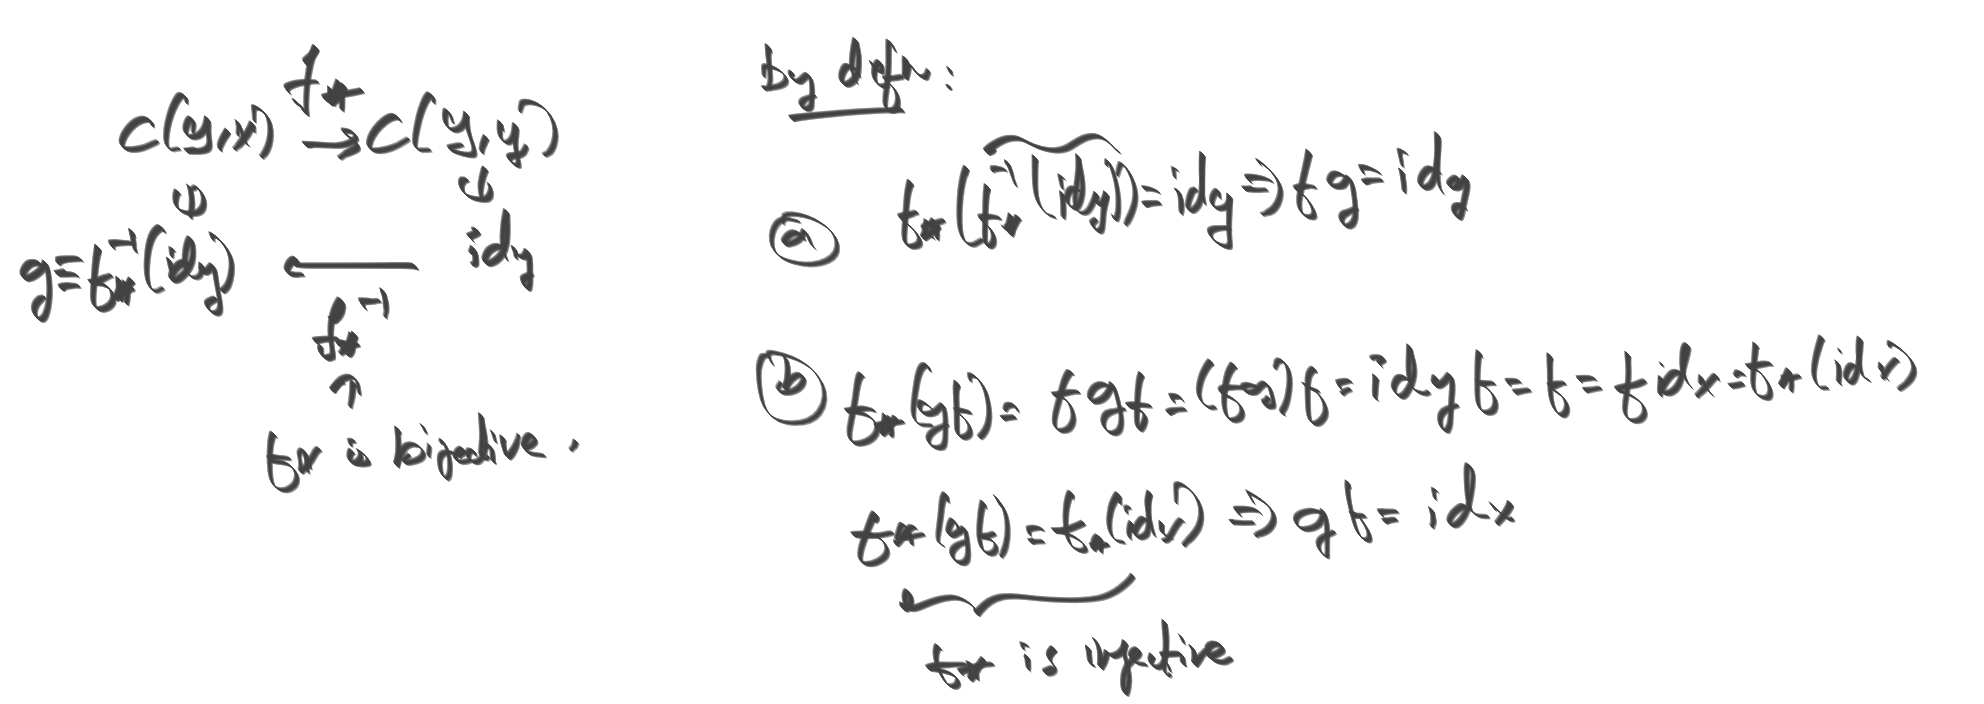
\includegraphics[width=\textwidth]{ch1/iso-is-bijection-of-hom.png}
    \begin{center}Iso is bijection of hom-sets\end{center}
\end{minipage}

\question{Q 1.2.ii:} Show that $f: x \rightarrow y$ is split epi iff for all $c \in C$, post composition
$f \circ - : C(c, x) \rightarrow C(c, y)$ is a surjection.


\beginproof[(split epi implies post composition is surjective)]
Let $f: e \rightarrow b$ be split epi, and thus possess a section $s: b \rightarrow e$ such that $fs = id_b$.
We wish to show that post composition $C(c, e) \xrightarrow{f_*} C(c, b)$ is surjective.
So pick any $g \in C(c, b)$. Define $sg \in C(c, e)$. See: $$f_*(sg) = fsg = (fs)g = id_b g = g$$.
Hence, for all $g \in C(c, b)$ there exists a pre-image under $f_*$, $sg \in C(c, e)$. Thus, $f_*$ is surjective
since every element of codomain has a pre-image. \qed


\beginproof[(post composition is surjective implies split epi)]
Let $f: e \to b$ be a morphism such that for all $c \in C$, we have $C(c, e) \xrightarrow{f_*} C(c, b)$ is surjective.
We need to show that there exists a morpshism $s: b \rightarrow e$ such that $fs = id_b$. Set $c = b$.
This gives us a surjection $C(b, e) \xrightarrow{f_*} C(b, b)$. Pick an inverse image of $id_b \in C(b, b)$. 
That is, pick any function $s \in f_*^{-1}(id_b)$. By definition, of $s$ being in the fiber of $id_b$,
we have that $f_*(s) = fs = id_b$. Thus means that we have found a function $s$ such that $fs = id_b$. Thus we are done.
\qed

\question{Q 1.2.iii:} Mono is closed under composition, and if $gf$ is monic then so is $f$.


\beginproof[(Mono is closed under composition)]
Let $f: x \to y, g: y \to z$ be monomorphisms (Recall that $f$ is a monomorphism iff for any $\alpha, \beta$, if $f \alpha = f \beta$ then $\alpha = \beta$).
We are to show that $gf: x \to z$ is monic.
Consider this diagram which shows that $gfk = gfl$ for arbitrary $k, l: a \to x$. We wish to show that $k=l$.

\begin{minted}{text}
    a --k-> x --f--> y --g--> z
    a --l-> x --f--> y --g--> z
\end{minted}

Since $g$ is mono, we can cancel it from $gfk = gfl$, giving us $fk = fl$.
Since $f$ is mono, we can once again cancel it, giving us $k = l$ as desired.
Hence, we are done.  \qed.

\beginproof[(If $gf$ is monic then so is $f$)]
Let us assume that $fk = fl$ for arbitrary $l$. We wish to show that $k = l$. We show this
by applying $g$, giving us $fk = fl \implies gfk = gfl$. As $gf$ is monic, we can cancel, giving
us $gfk = gfl \implies k = l$. 
\qed.

\question{Q 1.2.iv} What are monomorphisms in category of fields?

\beginproof Claim: All morphisms are monomorphisms in the category of fields. Let $f: K \rightarrow L$ be an arbitrary field
morphism. Consider the kernel of $f$. It can either be $\{ 0 \}$ or $K$, since those are the only two
ideals of $K$. However, the kernel can't be $K$, since that would send $1$ to $0$ which is an illegal ring map.
Thus, the map $f$ has trivial kernel, therefore is an injection, is left-cancellable, is a monomorphism.\qed


\question{Q 1.2.v} Show that the ring map $i: \mathbb Z \rightarrow \mathbb Q$ is both monic and epic but not iso.

\beginproof[$i$ is not iso]
No ring map $i: \mathbb Z \rightarrow \mathbb Q$ can be iso since the rings are different (eg. $\mathbb Q$ is a field). \qed



\beginproof[$i$ is epic]
To show that it's epic, we must show that given for arbitrary $f, g: \mathbb Q \rightarrow R$ that $fi = gi$:

\begin{minted}{text}
Z -i-> Q --f--> R
Z -i-> Q --g--> R
\end{minted}

implies that $f = g$. Let $fi: \mathbb Z \rightarrow R = gi$. Then, the functions $f, g$ are uniquely determined
since $\mathbb Q$ is the field of fractions of $\mathbb Z$, thus a ring map $\Z \rightarrow R$ extends uniquely to a ring
map $\Q \rightarrow R$. Let's assume that $f(i(z)) = g(i(z))$ for all $z$, and show that $f = g$.
Consider arbitrary $p/q \in \mathbb \Q$ for $p, q \in \Z$. Let's evaluate:
\begin{align*}
f(p/q) = f(p)f(q)^{-1} = f(i(p)) \cdot f(i(q))^{-1} = g(i(p)) \cdot g(i(q))^{-1} = g(p/q)
\end{align*}
which shows that $f(p/q) = g(p/q)$ for all $p, q$. Thus, we can extend a ring function defined on the integers to rationals uniquely,
hence $fi = gi \implies f = g$ showing that $i$ is epic.
\qed

\beginproof[$i$ is monic]
given two arbitrary maps $k, l: R \rightarrow \Z$, if $ik = il$ then we must have $k = l$. Given $ik = il$, since $i$
is an injection of $\Z$ into $\Q$, we must have $k = $l.

\question{Q 1.2.vi} Mono + split epi iff iso.


\beginproof[Iso is mono + split epi]
Iso is both left and right cancellable. Hence it's mono and epi. It splits because the inverse of the iso splits it. \qed.


\beginproof[mono + split epi is iso]
Let $f: e \rightarrow b$ be mono (for all $k, l: p \to e$, $fk = fl \implies k = l$)
and split epi (there exists $s: b \rightarrow e$ such that $fs: b \rightarrow b = id_b$.
We need to show it's iso. That is, there exists a $g: b \rightarrow e$ such that $fg = id_b$ and $gf = id_e$.
I claim that $g \equiv s$. We already know that $fg = fs = id_b$ from $f$ being split epi. We need to 
check that $gf = sf = id_a$. Consider:

$$fsf = (fs)f = id_b f = f = f id_e$$

Hence, we have that $f(sf) = f(id_e)$. Since $f$ is mono, we concluce that $sf = id_e$. We are done 
since we have found a map $s$ such that $fs = id_b, sf = id_e$.


\question{1.2.vii} Regarding a poset a category, define the supremum of a subcollection, such that the dual gives the infimum.
\beginproof We regard an arrow $a \to b$ as witnessing that $a \leq b$. First define an upper bound of a set $O$
to be an object $u$ such that for all $o \in O$, we have $o \leq u$. Now, the supremum of $O$ is the least upper bound
of $O$. That is, $s$ is a supremum iff $s$ is an upper bound, and for all other upper bounds $t$ of $O$, we have that $s \leq t$.
So we draw a diagram showing upper bounds and suprema:

\begin{minipage}{\textwidth}
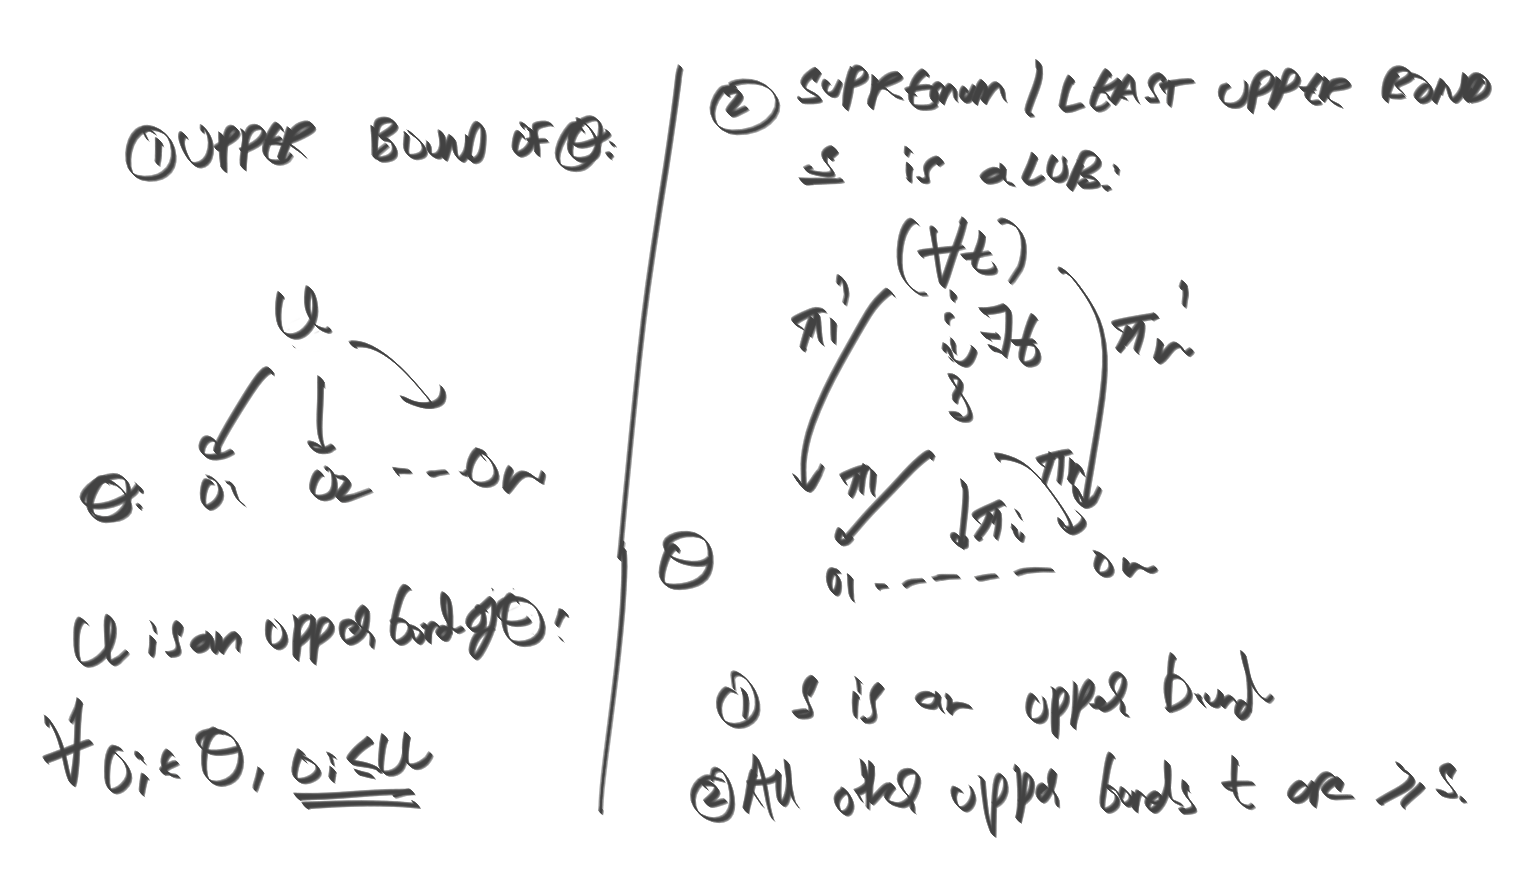
\includegraphics[width=\textwidth]{ch1/sup.png}
    \begin{center}Upper bound and supremum\end{center}
\end{minipage}

\end{document}
